\documentclass[a4paper,12pt]{report} % report, 12pt
\usepackage[utf8]{inputenc} % utf8
\usepackage{graphicx} % images
%\usepackage[pdf]{pstricks} %compilation pdf graphics
\usepackage[frenchb]{babel}
\usepackage[T1]{fontenc} % accents

\usepackage{fancyhdr} %en-têtes et bas de page
\pagestyle{fancy}

\usepackage{times} % Times New Roman
\usepackage{setspace} % interligne
\setstretch{1.15} % 1.15

%%\usepackage{hyperref}% pour le \url

%enlever le 0.1 du chapitre lorsqu'il n'y en a pas
\makeatletter
\renewcommand{\thesection}{\@arabic\c@section}
\makeatother

\renewcommand{\contentsname}{Table des matières}


\title{Rapport de Stage TN07 en \LaTeX \newline \newline
	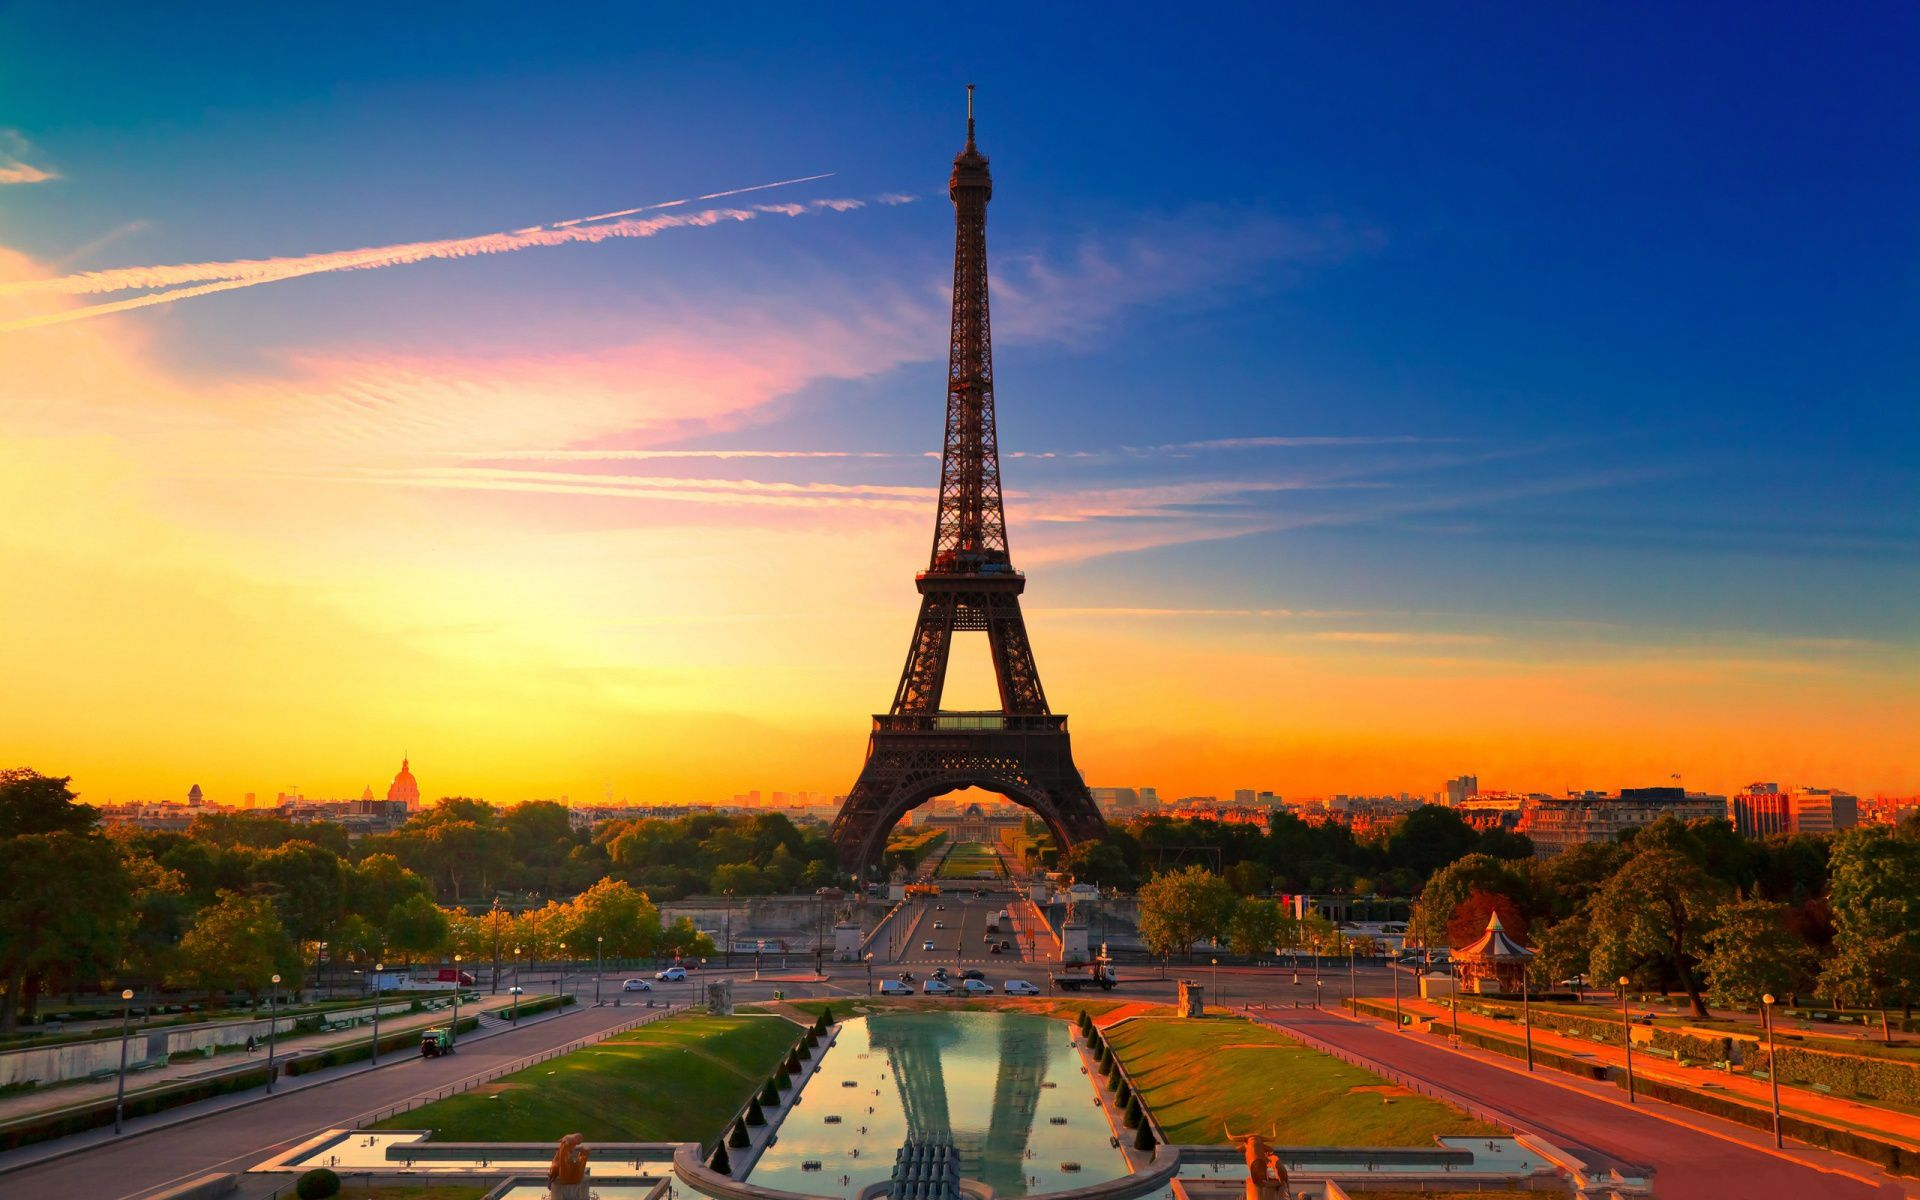
\includegraphics[width=\linewidth]{france.jpg}
}	 
\author{Grégoire MEUNIER, username : gmeunier}
\date{La date de rendu du rapport est le : \today}


%Definition des en-têtes
\fancyhead[L]{Grégoire Meunier}
\fancyhead[C]{17 septembre 2017}
\fancyhead[R]{Rapport TN07}	

\fancyfoot[C]{\thepage} 
\fancyfoot[R]{
\includegraphics[scale=0.2]{logo_utc.png}}


\begin{document}
\maketitle
\newpage % --------------------------------------------------------------------SOMMAIRE

\tableofcontents

%\newpage % --------------------------------------------------------------------Liste figures
%\renewcommand{\listfigurename}{Table des figures}
%\listoffigures

%\newpage % --------------------------------------------------------------------Liste tables
%\renewcommand{\listtablename}{Table des tables}
%\listoftables

\newpage% -----------------------------------------Intro
\abstract{Expecting from the trip}
\paragraph{I went to Finland to improve my English and to discover a new culture. I never went to that Scandinavian country except for Swedan, then my next step will be Norway ! The Scandinavian countries are part of the world that I would like to discover. You should ask me why ? Because since I was a child, my teachers always told me, and I read in newspapers that thoses countries have the best educational system in the world so I would like to figure out why.
As I don't speak the language of this country, the finnish, I have to write the report in English. Then, I think that my level in English speaking is the B2 level before I arrived. I used to travel a lot and that is why I have facilities speaking this language.}


\newpage
\part{Journal du séjour (in English)}% -----------------------------------------------------------------------Carnet de bord(8/9 pages)
					%--- 10/15 lignes par jour
\label{p:1}

\paragraph{Day 1 : Monday, 17 July 2017}
\subparagraph{I left Toulouse at 8:30pm in bus. I have a long trip which is waiting for me. I should arrive in Paris by 6:00am tomorrow ! Let's start to sleep a little.}

\paragraph{Day 2 : Tuesday, 18 July}
\subparagraph{Arrive in Paris at 6:30am. Actually, I didn't arrive to sleep. I now have to take the subway and join the CDG airport in order to take a plane which will bring me to Riga, in Lettonie where I will spend one day. I arrive in Riga at 2:00pm and go straight to my apartment that I've rented. It's a kind of big apartment where people all around the world could come and talk how they like to. Then I visited some historical buildings and what I could see is that the town is hardly marked from the independence war with Russia. After my three-hour trip around the city, I went to a restaurant, and there, I could eat food which was very special. In my first plate and my main course, they had put berries in there. I think they really like it ! Also the server was coming every five minuts to ask if everything was ok. People seems to be very kind there, after when I was coming back, it began to rain so I started to run to the tramway, and then when I was in front of it I remembered that it might not be free, and the driver saw me and told me to come inside despite the fact that I didn't have any ticket ! Then I went to bed because I didn't sleep so much last day.}

\paragraph{Day 3 : Wednesday, 19 July}
\subparagraph{Departure from the appartment at 5:30am. Arrived in Helsinki at 10:00am. When I arrived, I asked the driver of a bus which one should I take to go to the city center, and then he tried to help me, but his english was not very good so he called a girl, the only one, in the bus and she came to help me. Then he saw that the bus should go because of the time, so he told me to enter without any ticket, another time ! (it was like 10 euros !). Then I just went to a restaurant to eat before taking another bus to Lappeenranta, and I was shocked because the server asked me to pay before I ate, but it did not seem to be a fast food restaurant because he brought me the food to the table. I had four hours on the bus and then I arrived to Savitaipale. Another helper was waiting for me at the bus station, even if the house was just in front of the bus stop ! Then I entered and discovered the wife who hosted me, and she hugged me, I was a little surprise because I thought that contact was avoided when you meet somebody for the first time. She showed me her house and I met the five others helpers. She told me that here, we were like a family so I had to act in consequence of that. I appreciated it. Then I went to the sauna with others helpers. It was very weird to be almost naked with people I just met. But good experience, because I never went in a sauna before and in Finland, there is sauna in every house ! I stayed with others helpers and talked until midnight and then went to sleep.}

\paragraph{Day 4 : Thursday, 20 July}
\subparagraph{I started to work at 9:30 am. My job was to clean chairs and oil them in order to sell it after that. Then I sorted underwears for women and kids by size in the way to sell it too. It was very strange as a mission for my first day of work. After I completed my job, friends of Sofia came and asked me if I would like to come with them play Frisbeegolf. It's a sport very well known there, so of course I accepted. Then we went there and I very liked the game ! I hoped they will come back another day in order to play with them again. The food was not very healthy I think, but Sofia doesn't have so much money so we have to deal with that. But even, she manage to put berries in our yogurts ! It's an obcession here ! After diner, we played a game (Dixit), and I was surprised that the Argentinian man doesn't know the sentence "Where is Bryan ?", I thaught it was a legend known all around the world.}

\paragraph{Day 5 : Friday, 21 July}
\subparagraph{Today, I brushed some toys, I passed sand papers on skillets, then I put oil on a big wooden table in order to make it great again. And today, it was the first time that almost five people answered me when I told them "Hi" ! I thought that nobody ever says "Hello" to strangers, but, in fact, I don't know... During my work, I walked around the bulding with the speaker in my hand while I was listening to music and a child, almost 6 years old, told me that the speaker was a good one. I was surprised that a little guy like him could talk to strangers so easily -- very different from older people. Then a old women on the terrace of the fifth floor of an appartment asked Davide, the Italian man, who was cleaning carpets to take her clothes which had fallen on the ground and put it back on the clothes line. I don't know if it was by laziness or if it is in the Finish culture. It has been two days that Sofia doesn't eat with us because that she has to take care of the shop so she stays closer than we are.}

\paragraph{Day 6 : Saturday, 22 July}
\subparagraph{Today, we went to the cabin. It's a second house, near a lake, which has no electricity and no running water. There, you just relax and have good times. And, of course, there is a sauna in every cabin, but not an electric one, this one is with real wood and rocks. In Finland, there is a tradition about Sauna because they used to use it for deliverys because they were not so much bacteries inside and it still warm, and that is a good point for the baby. And then, to clean a body when a person died. You start and finish you life in sauna in Finland. But why only here ? Maybe because they have a lot of trees ? I've never seen a country which has such a numbers of trees everywhere ! It's really amazing !}

\paragraph{Day 7 : Sunday, 23 July}
\subparagraph{I painted the outside of a room during the whole morning. And during the afternoon, I went in the forest with my Argentinian friend. We saw a place where all the trees were cut, but only one was still there, in the middle of a dead plain. My friend said that it might be a sign done by owners to say that it's their properties or something like that. On our three-hour trip, we saw some cars and every person inside the car was saying hello by waving to us. Maybe because it's not the city, then people feel more relaxed and calm. We did a barbecue for dinner. It's the same as in France, only that they have a kind of donut without sugar but with meat inside. It's delicious! After that, we played Mölkky (say 'melke'). It's a Finish game which is so close to bowling, but with wooden sticks and it's outside. In fact, that game is really well-known in France. I used to play it when I was in Toulouse.}

\paragraph{Day 8 : Monday, 24 July}
\subparagraph{I finished the paint during the morning. Then, during the afternoon, I went to the lake with the boat. Actually, it's not a lake because it's size is smaller than 1km. In Finland, there are more than one hundred thousand lakes, then you can imagine how much there will be if we count even thoses water points which are like that one, which is not that small. There are enough water points in order that everybody can have a cottage. During my excursion, I saw numbers of boats which were given up around the lake. In the late afternoon, the Sofia's sister with her two children arrived at the cottage. After dinner, I was very surprised that Laura gives salt snacks to her children as a dessert. We used to eat it before starting the dinner in France. I was quite surprised.}

\paragraph{Day 9 : Tuesday, 25 July}
\subparagraph{During the afternoon, we played a game with the two kids. In fact, they don't speak English, or only a few words, but they still have seven and eleven years-old, so it remains the same as in France. But actually, the Heikki's brother, who was playing with us FressbyGLof last time was perfectly speaking English, and he is only 13 or 14 so he has a good level for his age. But then, the bad thing was that as the two boys do not speak English, the entire family had to speak in finish, so we were not speaking all together at all like it was before they arrived. After that, we went to the sauna, a real one, with wood. Inside, the temperature is about 90°C and the tradition is that after being in the sauna for about 10 minutes, we plunge inside the fresh water of the lake. It had been a really good experience ! When you stayed standing up outside after sauna, you can even see the heat leaving your body.}

\paragraph{Day 10 : Wednesday, 26 July}
\subparagraph{Today, we leave the cottage, so we have to clean before we go. We spent a lot of time, tidied up the Mika's warehouse because it was a big mess. We ate just before to leave the cottage and I was very frustrated when someone Finnish, who I will not write the name here, took the last piece of meat without asking anybody around. I taught that was just rude, but in fact, I could have seen while checking around that nobody was upset, so I figured out that it was a French manner and not an international one. Then we took the taxi to come back. The cost of the taxi was about 120€ to go and the same to come back. And Sofia goes like every 2 weeks in the cottage, and every time she pays for everbody! It's a big amount of money that she spend for us, just wonderful.}

\paragraph{Day 11 : Thursday, 27 July}
\subparagraph{I noticed when I arrived that the bread they used to eat exits in different kind. They have the white bread, which is "pain de mie" in France, and they have also a black bread. I never saw one of that kind in France, but don't really like, it's drier than the white one I guess. Also a specific thing that I only saw in foreign countries, during the dinner, they always cut the cheese with a special knife, so it was a quite disappointed feeling for a french guy like me who used to eat the cheese in a plate, with different knifes for every kind of cheese and not even in the plastic bag. In fact, after several days in this coutry, I can really see that there are numbers of cultural differences.}

\paragraph{Day 12 : Friday, 28 July}
\subparagraph{Today, I met the second Sofia's assistant, she came back from holidays. It's now the time to say that the manner to say "Hello" in France is very different. In Finland, we just shake hands for the first time you see somebody, Mens or Womens, and then, for next meetings, you just say "Hello" without any contact. Whereas in France, womens between them kissed, and even women with men. Then, I went to the S-Market to buy some things we needed. I was disoriented during that time because on all Finnish products, it is written in 3 languages : Finnish, Swedish, Russian. But not even in English. It's written in Swedish because in the north, near Sweden, most of the people speak Swedish then that's why we have this language on the product. And for the Russian, on the East cost, there is a long border between Finland and Russia.}

\paragraph{Day 13 : Saturday, 29 July}
\subparagraph{Because it is the end of the week, I discussed with Sofia about some hours I did. When we were in the cottage, I found a chair that needs to be put on a tree. Then I figured out that it needed to be done. Even if I had already finished my work for the day, I was not so tired so I continued. I asked Sofia about where to put the chair, how to put it on a tree in order that she can use it afterwards. But today, she told me that the hours, more than 2 because it was above the water, I worked with the chair was not taking into my daily hours because she did not ask for it. I thought it was really unfair, but I did not say anything because she manages the work so I think that I have not the power to decide.}

\paragraph{Day 14 : Sunday, 30 July}
\subparagraph{Since I was here, no one robbery was committed in the Sofia's house, even outside. That despite everything she sells is outside with no cameras. Even bike, free to be stolen, but finish people trust them and are sure that nobody will steal anything and this is the reality ! I find it unbelievable ! In France, we need lockers for a single thing, and here, you have more than 600€ of stuff outside and nobody care. I really like this manner of thinking. Believe in your neighbours and other people is the thing that needs to be achievable once in a life. For lunch, Mika did for the third time his wonderful soup. It's obvious that he has special skills for that kind of food. His food is delicious, I think that I have never ever eat a better soup.}

\paragraph{Day 15 : Monday, 31 July}
\subparagraph{The thing that you are glad to have here in the shop is the miraculous sponge. It's like a normal one but white and it's a kind of sandpaper, but a very soft one. And when you have that for cleaning, you are the oil magnate. In Suomi\footnote{Finland}, as we are far in the north, the sun doesn't go down too early. He might stay until 11:00pm! And in the morning, he wakes up very early! If you don't have curtains, it's very hard to sleep well. But in spite of that, they still have kids in the late evening who are doing motorbikes making a lot of noise. They are a crew of 4/5 persons, and they go around the city during at least 2 hours. We have the same guys in France I told Sofia!}

\paragraph{Day 16 : Tuesday, 01 August}
\subparagraph{Today, Mika drove me to Lappeenranta. He had to go to the other shop they have there so I could bring me with him. When I arrived, I walked about 2 hours across the city. The city was calm and peaceful. There were not so many people, it was pleasant. Then I went to the harbour, I saw a lot of boats. I really like boats, we feel like we can travel all around the world inside and even live on it. Then, I saw architectures made with sand. The city of Lappeenranta made a story wih that sand like they hope it will be in their future. I could spent some times in the park. Reading with no one around. Very peaceful. And my last step was shopped. I needed a coat and I guess that in Finland, because of the time, they should make better winter clothes. I found a really good one, very cheap, and then, I can tell you that I am not cold at all inside!}

\paragraph{Day 17 : Wednesday, 02 August}
\subparagraph{Once more work day, but on this one, we have a new helper with us ! Ruth from North Carolina (USA) arrived in the late afternoon ! This is good to speak with someone who takes your knowledges into account. I mean that she speaks slowly and could repeat several times if we still do not understand. Not the same like Jamie from Manchester (United Kingdom) who speaks very fast and in an unintelligible way. Very hard to understand. She explained us, to the helpers, that she is a nurse and in her job, she has to explain to foreign people what they should do to keep a good health, then she should be understood, that's why she learnt how to manage to speak slowly and clearly. She likes to travel and me too, then we went to a museum near by. We could see ancient items from the past fews centuries. Then we came back slowly to the house.}

\paragraph{Day 18 : Thursday, 03 August}
\subparagraph{I showed Ruth the house, and explained her the name of each rooms we have in the house, because we have a lot ! During the dinner, as Rith was just arrived, she stayed longer with us and told us a story, her story. When she bought this house, it was a bank. That's why we have a room called "The Jail", because there is still the big door which was here to protect the money. Then, she made a restaurant with that place. It was a really good one. But with the time, she become sicker, then she decided with Mika to stop the restaurant. Then, they started to sell every items they had, because it costs a big amount of money. But then, they continued to sell again and again, so they started a second hand-shop. That's how Pillipu was created.}

\paragraph{Day 19 : Friday, 04 August}
\subparagraph{On that day, we have Kamila and Psemeck who arrived. They are from Poland. I am glad of that because I might go to Poland for a 6 months intership next year and then I could speak a lot with them about the cities, universities, about the life there, the ambiance, the cost, and plenty of other things like that. I learned that the AGH University of Science and Technology is one of the most famous uniersity in their country. And the UTC has a partnership with them. But I can't do Informatics there so even with thoses informations, I will not be able to go there. Then now, we are 10 helpers ! And 3 others are coming tomorrow, and it's obvious that the table will not be long enough to let everybody eat on. We will see how managed that.}

\paragraph{Day 20 : Saturday, 05 August}
\subparagraph{Gael, Philippe and Cesar, from France just arrived today. There are also from an engineer school but near Le Mans. In there school, they don't have to do an intership but they have to go at least 8 weeks in a foreign country. I don't know if it's good to go "vacations" with one's friends abroad. And what about people who can't afford a trip like that one ? Then we played Mölkii all together. We could see that Japanese people have special skills for that game ! Narumi was really good to earn a lot of points ! Then, we played but not all together at a game called "Times'up". The goal is to explain a word without saying it to other people and they have to find the word ! It was a really good exercise for my english practice.}

\paragraph{Day 21 : Sunday, 06 August}
\subparagraph{Today was a sunny day, so with Ruth and Mia, we went to the field of strawberries pick up some of them. We had to pick up 20kgs, but in fact, after more than 2 hours of fast picking, the field was over, and we could not have more berries than we got, and it was only 7kgs. Afterward, it was obvious that we had to wait until the next sunny and at least 3 days in order that green stawberries could become redder. To go there, we used the Mika's van. I drove to bring us there. In that way, I could see that the road's rules are not the same as in France. On a big road, you can drive until 100km/h, but on a little one, even outside of the city, you are limited to 60km/h, as in the city. I also saw that people are very respectful on the road. Nobody was following me too close, very different from France where people just come closer in order to make you go faster.}

\paragraph{Day 22 : Monday, 07 August}
\subparagraph{Today, we went on a 30 minuts trip to go to a restaurant. In that one, you can only eat "Lemin Särä"; the oldest traditional food in Finland. It's a plate with mutton and potatoes. There, you can eat which quantity you want ! There is even a record ! 11 plates. I could only ate a little more than 4, but it's not that bad ! The meat is heated up in a deep oven. Years ago, they even used to sleep near by because the temperature was very high and during the winter (even in the other seasons), it's very cold ! We also drank a weird thing. In fact, I did not like it. And as a dessert, is was a kind of sound with graps and peach, but I did not like it to. The taste was really strange and mixed up everything like that was not usual for me. As we went, we came back in a bus and during the week, that bus is used to drive children to school, so the driver had to blow inside an alcotest if he wanted the bus to start. I think that thing should be in every car and in every bus ! Very useful to be sure that we can drive safely !}

\paragraph{Day 23 : Tuesday, 08 August}
\subparagraph{On that day, we went on the beach. In fact, it was not a beach, only a space with sands near a lac, as always in Finland as you know now. There were nobody only us, it was almost calm. Yes almost because we were more than 10 people then it cause some noises. We could use a barbecue there. And the wood was already cut. So we could use it without any permission. Afterwards, I am wondering myself who should have cut that wood, but I did not asked. It still strange here in Finland how it works.}

\paragraph{Day 24 : Wednesday, 09 August}
\subparagraph{Sofia told us something while we were eating. In fact, currants came from Finlande. They used to make wine with thoses one. It was imported in France during the Middle Ages. We were wondering why here in Finland they always eat berries. She answered us a simple thing, they only have berries in Finland !}

\paragraph{Day 25 : Thursday, 10 August}
\subparagraph{In a normal group in France, when there is a blank during the conversation, it causes embarrassment among ppeople. But here in Finland, it is almost normal, because they speak only when they have something to say. Another story of Sofia : an american teacher was asking "how are-you ?" to everybody as we used to in the USA, and people were explaining their problems in their life because they were thinking that he really care about us by asking that ! It's just a difference of culture.}

\paragraph{Day 26 : Friday, 11 August}
\subparagraph{Mika needed me in Lappeenranta, then we left the house after lunch. There, we had to reorganise many stuff in a shop. In fact, that shop is a big second-hand shop. People rent a piece of space in that shop, and bring stuff in the way to sell them. In exchange of that space, and the administration of the sale, the big shop takes 20\% for each sale. After our job was done, we went to the bakery. It's different from France, there it's in self-service. You just come, and take what you want, and then pay.}

\paragraph{Day 27 : Saturday, 12 August}
\subparagraph{I went for a walk. In front of each house or each appartment, you can see a thing that is used to clean carpet. I though it was only in front of our house but it's not true ! You have even that other thing that is used to clean your shoes before enter in a house. There is in fact a social habit in Finlande to have the possibility to clean everything. And to continue in thoses specials things, every door has its locker in a different way than in France.}

\paragraph{Day 28 : Sunday, 13 August}
\subparagraph{If you climb a roof in a Scandinavian country, you should see a ladder on each roof. It is almost mandatory to have it because during the winter, the snow is everywhere and you need to take that off because if it falls on its own, you can died by being above. Winter season is said to be very different from summer one. I should come back another time to see it because I had not see the snow in Finlande yet.}

\paragraph{Day 29 : Monday, 14 August}
\subparagraph{That time, I did not miss the fire brigade's alarm which was ringing. I thought I heard it last monday but as I was not sure, I just waited another monday to confirm what I heard. In France, it is on the first wednesday of each month.}

\paragraph{Day 30 : Tuesday, 15 August}
\subparagraph{I went in Mikkeli with Ruth. It is a one hour trip from Savitaipale. We planned to spend a day in Mikkeli, then go to Savonlinna where a castle was build many years ago, and sleep in Savonlinna in our tents. In Mikkeli, we visit a big church. There was an organ in that church, but not in front as most of the french church but elevated at the back. In fact, it was the same for the three churches we visited. We also noticed that stained glasses were deprived of painting.}

\paragraph{Day 31 : Wednesday, 16 August}
\subparagraph{The night is Savonlinna was very hard. The temperature was very cold, and the city very noisy. Very hard to sleep in such conditions. But despite of that, we did not pay anything so our trip was very cheap, only the food and the bus ! And it was a real natural finnish experience ! We packed our stuff and started to came back to the city center in order to take our bus back to Mikkeli the Savitaipale.}

\paragraph{Day 32 : Thursday, 17 August}
\subparagraph{We rest one day in the house, and after that, Sofia planned to go to the cottage, but that time, with everybody ! We went there at 9, too much people but really fun. Sofia thought about staying there five days. Me and Ruth needed to came back on Sunday because we had to take our bus to Helsinki in the early Monday. The plan was that Sofia's sister should came to take us on Sunday.}

\paragraph{Day 33 : Friday, 18 August}
\subparagraph{In the same way as in the house, everybody has a task to do. Mine was to clean the lake. Not everything of course because it was to big but just a side of the lac, neer the cabin. Philippe helped me in that task. It seemed like everytime we cleaned a part under the water, it went dirty afterwards in seconds. After too many years, it was almost impossible to clean that giant lake by hands.}

\paragraph{Day 34 : Saturday, 19 August}
\subparagraph{On the first day, we used to threw the dirtiness on the shore, but used the bark was in fact a better option. We put the tarp in that boat and just threw everything inside. Sofia asked us then to throw everything further on an other shore. I do not know if it was the best option or not but it was what she wanted, so we had to do that.}

\paragraph{Day 35 : Sunday, 20 August}
\subparagraph{I noticed that finnish people has a very strang manner of pronouce things. As exemple, when I was talking with Mika, he told me a french brand of car. He pronounced it like : "pé-u-jé-aut". When you thing and read it, it is obvious that he was talking about Peugeot, but that manner of pronounced every letter that you see is very different for French people. But it is the same in many languages. We came back to the house in the late evening.}

\paragraph{Day 36 : Monday, 21 August}
\subparagraph{We left the house, after more than a month spend in it. We left the house together Ruth and me so it was easier than if we had been alone. We took the bus to Helsinki }

\paragraph{Day 37 : Tuesday, 22 August}
\subparagraph{I spent the day in Helsinki, visinting many different places. We even stopped in a library. There were books from a time too far to even say ! It was a pleasure to spend that time in that big city.}

\paragraph{Day 38 : Wednesday, 23 August}
\subparagraph{Last day in Helsinki, and also in Finland, it is the time to end this fabulous trip into another culture.}

\newpage
\part{Présentation de l’organisme et du travail effectué (en français)}%----------------------------------------------Présentation (2/3 pages)
\label{pt:2}
\paragraph{\underline{Nom :} \newline \textbf{Sufoon Ky/Pillipuun puoti} \newline
\underline{Adresse :} \newline \textbf{Peltoinlahdentie 23  54800 Savitaipale FINLAND} \newline
\underline{Site web de l'entreprise :} \newline \textbf{https://www.facebook.com/Piilipuu/} \newline
\underline{Date précise du stage effectué :} \newline \textbf{19 juillet jusqu'au 23 août} \newline
\underline{Domaine d'activité de l'organisme :} \newline \textbf{Magasin de produits de seconde main, d'occasion.} \newline
\underline{Organigramme, place du stagiaire :} \newline \textbf{Pour expliquer, je vais utiliser des mots propres à une entreprise, même si les relations que l'on avait n'étaient pas les mêmes qu'en entreprise. Sofia était la manager de l'entreprise. Elle avait deux salariés à temps partiel dans la semaine pour l'aider dans ses tâches, ainsi qu'une dizaine de stagiaires (helpers) non rémunérés mais nourris, logés.} \newline
\underline{Organisation de la journée de travail du stagiaire, tâches accomplies :} \newline \textbf{La journée commence entre 9h et 10h suivant les jours, et se déroule jusqu'à 15h ou 16h, le repas n'est pas compté dans les horaires. Je faisais 5h de travail par jour et 25h par semaine. Les tâches étaient très diverses et variées mais la plupart du temps consistées à nettoyer des objets qui seront par la suite vendus.} \newline
\underline{Réflexion sur les comportements au travail :} \newline \textbf{Sofia nous donnait une nouvelle mission dès que la précédente était terminée. Nous étions autorisées à prendre des pauses n'importe quand. Le comptage d'heures de travail devait être fait par nous même est été basée sur une confiance total, Sofia ne verifiait jamais si l'on trichait ou pas. Cela rendez donc le travail beaucoup plus facile et libre.} \newline
\underline{Réflexion sur les relations au travail :} \newline \textbf{Les relations étaient très bonnes et faciles puisque Sofia vit avec tous les helpers le reste de la journée, donc nous étions tous amis avant tout.}}



\newpage
\part{Etude interculturelle (en langue étrangère)}%------------------------------------------------------------------Étude (12 pages)
\label{pt:3}

\section{Confidence}
\paragraph{When I arrived, I immediately saw that there were so much bicycles in gardens, without any lockers or any surveillance. But more astonishing, Sofia's shop stayed open with everything outside during all the night. I asked myself, why Finnish people are so confidente with their neighbors while we are not at all in France ? Even in a safe place with a locker, I got my bike stolen during the first week I stayed in Compiegne, my studied city. Obviously, thieves of Compiegne would be so happy to come in Finland. According to Statistics Finland's preliminary data, a total of 364,800 offences were recorded by the police, customs and border guard in January to June 2017 while we had more than 3 millions crimes and misdemeanors recorded by the police in 2016. How explained that ? After several researchs, I must say that we don't really know why it is like that, it is like it has always be like that. Almost anchored in everybody's mind. The only point we can rise is that in France, we had manifold wars during the twentieth century, and in different places around the world meanwhile Finland had only a few wars and it was mostly inside their own country. I mean that inside war put people closer between them, and outside wars does not change anything. Then it seems to be now how it was during the war, you can trust your companions, and you have to. So they believe in others, and it make their lifes easier ! 
In the 80's, Finland is one of the country with the lowest rate of unemployment. It remains like that during almost 10 years. They never had to blame somebody else for a bad rate. Then they should have been closer than we are in France. That might explain why they are so confident between each other.
An other point we can add is that Finnish people do not have the time nor energy to spend about social issues, they just do what they want to. As an exemple, I can tell that I never saw a country before with more people with colored hairs. Purple, orange, yellow, you can see a real rainbow of hairs in Helsinki ! A lot of people have also tatoos, when in France, most of the time, people prefer hiding it below their tee-shirt. \newline
\textit{Du rififi chez les hommes} (1955) by Jules DASSIN was banned from cinemas because inside the movie, you could see a perfect robbery of a bank. The governments of Finland, at the end of the 50's, thought that this movie, could give thoughts to the population, as an exemple, a person who would like to be a copycat of an actor in this movie. In order to prevent it, they prefered to ban it. I do not know if it was the best option, because human is alway attracted by forbidden things. It also shows us that at this time, the gouvernement was not very confident towards its citizens.}

\section{Way of talking}
\paragraph{Finnish people has a special manner of doing, talking. Or maybe Scandinavians in general, but that hypothesis would need further reseash and trips to prove it. To come back on the Finnish, they describe themselves as people who speaks only when they have something to say. You do not talk because you see somebody you know or something else, you talk because you need something or need to ask something. \newline
We can come back on the story of the american teacher who ask "How are you ?" to everybody; He was lost in that country because he had kept his own habits from his country and did not adapt himself to that new country which he did not know anything for sure. Another story, is that a man knocked at the door of his neighboor, the latter opened and offered him a cup of tea. That same man continued to talk and after a moment, asked the first guy if every thing was ok in his life. The other man answered that to be honnest, not really, because his house was burning. It is a simple demonstration of how it is in Finland : the courtesy is the queen of everything. \newline
The suomi, the Finnish language seems to be very differente from the French. Firstly, the pronunciation is not the same. As many languages, they used to pronunce every letters in a word, when in France, we can write letters but do not pronunce them, liek the "h" for example. It is that kind of letters that you write down but never say. \newline
In Finland, you do not need to talk to understand or communicate. If you are lost in the city, you just have to find a person, and even that one does not speak a language you understand, she will try to endeavour. \newline
A thing that really stands out in my mind is that word : "Noni". I will not explain everything but you can watch that video in order to understand what I am going to tell you : \textit{Suomen Ismo Leikola} by Ismo Leikola. With only one word, you can answered at more than ten sentences ! That works because they change their manner of saying it. You have to have a higher voice or a louder one, change your ton, ... And the meaning of your word can change ! \newline
A point that I thing is not really different is that old people do not use to speak English. I mean that most of our grand parents are not really used of English, despite the fact that most of the young people are learning it at school. It seems to be the same in Finland, when I was talking to old people, they were not understanding me, and they were answering in Finnish. \newline
The way you say "hello" in France is very different from anywhere in the world, and then especialy from Finland. This practice depends completely on which part of France you are visiting. For example, the number of kisses you do varies from 1-4, the action of greeting can start from left or from right side of the face, and women kiss both men and other women, but usually men do not give kisses to each other, except when they know each other for a long time. In Finland, a simple "Hey" or "Good morning" is more than enough.}

\section{Mentality of recycling}
\paragraph{Compare to France, I believe that there is a real movement from the government against the polution and the accumulation of waste. Even the population get into it. A simple example, the place were I was, a second hand shop. If I would like to describe it for a French man, I should say empty-attic, a vacuum-attic, a secondhand trade, .. but a permanent one. And if you think that this activity is marginal, you are completely wrong ! You can see more advertising of second-hand shops in the city than anything else ! They are creating a new field of activity that should come through the Europe up to France. You can say that we have already that kind of shop in France, but I will just answer you that the number of shops is not comparable in both coutries. When you manage a second-hand shop, you need a lot of patience and spaces because you buy a big package of stuff at a low price and you sell each thing alone, and when you sum up the price of each thing alone, you can see that you earn more monney than you put to buy the entire lot. The goal is to buy many different lot, and wait until people buy everything. Something, you will need a lot of time because people do not want every objetcs you can have, then you need to keep them in your house if you do not want to throw them. \newline
Wereas in France we just throw cans in a simple bin, in Finland, you pay more to buy your drink when they are inside a can, but then, if you gave them back, they gave you back your money ! A system like that is not too difficult to set up, and after that, cities's waste will be empty. \newline
The first day, when I arrived, in Helsinki, I noticed right away that people were allowed to take everything they need from bins when I saw three mans scouring bins. It seems to be a good thing, but hard to say why we can see it more here than in France. In France, the law says that you are allowed to take things from the bin, but if you get ill, you can say that you were poisoned by the person who put the waste in the bin. Then in the way to do not be annoyed, people or companies can put bleach in order to deter people for scouring inside your bin. Sofia just says that it is normal that people can take foods that others do not want or can't sell. And it seems to be everywhere the same in Finland because companies used to put foods that they do not want in a different garbage bag than hazardous substances. Actually, you can also find some companies who do that. As example in Compiègne, several bakery give their unsold stocks at the end of the week. If everybody who has over food than needed used to give it and do not throw it, the world would be a better place. \newline
A reason why people are so involved in recycling might be because products like beer, electricity, water cost more than anywhere else. Even the life in general is more expensive. In the way to earn money and spend it in useful things, people would have like to save it then they take care of things and know the real value of money. But this is just a guess, maybe not the reality.\newline}

\section{Foods}
\paragraph{Whereas in Finland, having an aperitif might mean drinking a small shot of whiskey before heading to the table, the French prefer to gather together with their friends to drink a little glass of wine before the dinner. Also, it is important to not to forget to enjoy your drinks with some small salty snacks, for example olives, salted peanuts, chips or other "gateaux apéritifs" as we say in France. The pre-drinks can end up during a few hours and include a lot of cheering and interesting discussions while in Finland, there not really used of that.\newline
As we all know, French people love their baguette and get it fresh from the bakery every day. Actually, it is one of the most important parts of their diet. Do not forget to buy a small mountain of bread if you decide to cook dinner and invite your French friends over, otherwise they might be shocked. In contrast, in Finland, they do not need a fresh bread, but soft bread is enough to satisfy them. The specificity is that they have different type of bread. You can find the white bread, the one that is the most close to the French one. You have also the black one, harder than the other, you can eat it with the same products as the white. And the last that I saw is the sweet bread. Very strange when you eat it for the first time, but then you get used to it (if you like it, and that is not sure !).\newline
France is the reference from cheese. In Finland, they sell it, but as a French guy, I should tell that it is not the same quality. The prices remains the same but unfortunately, not the taste. \newline
But as a normal civilisation, they should have they own speciality. If you go in Finland, you will be able to try reindeer meat. There is restaurant which are specialize is that kind of food as I told you in part~\ref{p:1}. \newline
One more thing that might shocks is the difference between the Northern and Southern Europe’s breakfast culture. First of all, in Finland it is very used to have the breakfast salty and they are said to consider it as the most important meal of the day. This means that it has a considerable amount of their daily energy intake. You can find for example sandwiches, boiled eggs, oatmeal, yogurt or cereal on a Finnish breakfast table.
On the contrary, a French person will like his breakfast sweet and light, or will completely skip it. An ordinary breakfast would be for example, cake, croissant, toast with jam, bun or chocolate bread. Just be careful for not to eat too much to have space for lunch! One thing in common with these two cultures is that coffee seems to be the drink that keeps us all agree. \newline}


%Another tip to show you are enjoying your dinner is to wipe your plate carefully at the end. According to my trustable French source, it might even be considered impolite if you forget to do that, as wiping the plate is thought to be a sign of enjoying the food.%

\newpage
\part{Capitalisation de l’expérience TN07 à l'étranger (en français)}%-----------------------------------------------Capitalisation (2 pages)
\label{pt:4}
\paragraph{Stage TN07 \newline
Nom du stagiaire et date du stage : MEUNIER Grégoire du 19 juillet au 23 août\newline
Pays : FINLANDE\newline
Ville, situation géographique dans le pays, nombre d’habitants : Savitaipale, 4h de Helsinki la capitale, au Sud. Moins de 5000 habitants. \newline
Organisme : Pillipuun puoti\newline
Secteur d’activité, nombre de salariés : Magasin de reventes d'objets d'occasion, un couple de patron, deux employés, une dizaine d'helpers.\newline
Nature du travail effectué, rémunération : Nettoyage, réparation, rangement, .. contre nourriture, logement, lessives\newline
Bilan de l’expérience professionnelle : Tâches professionnelles n'apprennent pas beaucoup de choses, mais montre la manière de fonctionnement en Finlande d'un travail.\newline
Conseils pour la recherche de l’organisme : Utiliser des sites tel que Workaway, helpex, woofing, .. Ou bien postuler directement sur le site d'une entreprise, local ou nationale.\newline
Formalités, visa : Pays de l'union européenne donc pas de visa à demander, seulement la carte européenne d'assurance.\newline
Hébergement : La maison étant mélangé au magasin, nous dormions juste à côté.\newline
Adresse, prix : Peltoinlahdentie 23  54800 Savitaipale FINLAND, gratuit puisque c'est en échange du travail\newline
Conseils pour la recherche de l’hébergement : Voir auprès des étudiants si vous ne passez pas par workaway ou un site comme ça.\newline
Conseils divers pour bien profiter du séjour : N'hésitez pas à revoir votre anglais, et à apprendre les mots basique en finlandais, bien que l'anglais vous suffira amplement.\newline
Manifestations culturelles : Voir calendrier de la ville.\newline
Transports : Omnibus le moins cher.\newline
Achats… : Attention aux prix qui sont en général plus forts qu'en France.\newline
Conseils pour réussir son intégration : Rien de particulier, il s'agit avant tout d'un pays européen.\newline
Pièges interculturels à éviter : Ne soyez surpris de rien, n'hésitez pas à demander, et restez ouvert d'esprit, tout se passera bien ;)\newline
Clés de réussite : Parlez avec le maximum de gens, demandez leur leurs histoires, questionnez les sur les différences interculturelles, .. profitez au maximum de cette échange !\newline
Pour plus d’info, contactez gregoire.meunier@etu.utc.fr\newline}

\newpage % ----------------------------------------------------Bibliographie
\part{Bibliographie}
\label{pt:5}

%\bibliographystyle{plain} 
%\bibliographystyle{abbr} pas utilisée
%\bibliographystyle{alpha} pas utilisée

%\bibliography{biblio}
\paragraph{\url{http://stackoverflow.com/}\newline
http://www.stat.fi/til/rpk/index$$\_$$en.html\newline
\url{https://www.inhesj.fr/fr/content/rapport-annuel-2016}\newline
\url{http://www.freegan.fr/loi_poubelles.php}\newline}

\end{document}
